\documentclass[a4paper,11pt]{article}
%\usepackage{stdpage}
\usepackage{microtype}
\usepackage{tikz}
\usetikzlibrary{calc}
\usetikzlibrary{through}
\usepackage{tgpagella}
\usepackage{subfig}
\usepackage[utf8]{inputenc}
\usepackage[unicode,breaklinks=true,hypertexnames=false]{hyperref}

\definecolor{mylinkcolor}{rgb}{0,0,0.5}
\hypersetup{%
   colorlinks=true,%
   linkcolor=mylinkcolor,%
   urlcolor=mylinkcolor,%
}

\begin{document}

\vspace*{3cm}

\begin{center}
{
    \huge Games for a multi-touch table

    \vspace{0.5em}

    \large IT project – Component Description
}

\vspace{3em}

Petr Viktorin

University of Eastern Finland

2011
\end{center}

\vspace*{2.718\fill}

\newpage

\tableofcontents

\newpage

\section{Summary}

This document describes the implementation of two games for
multi-touch tables, Maze and Towers, a utility for replaying past games to
help analyze players' behavior, and a multi-touch table built for testing the
games.

The reader should get familiar with the User manual for the games before
reading this documentation.

\section{System description}

\subsection{External Libraries and Supporting Software}
\label{dependencies}

The multi-touch games use several pre-existing pieces of software to work.
This section describes these prerequisites.

\subsubsection{Python}

The games are implemented in Python, a dynamic, interpreted programming
language designed for code readability and ease of development.

The games were written using Python version 2.6 and are compatible with
the current version, 2.7.

The games are not compatible with Python version 3, as some libraries (notably
Kivy) do not yet support it.

\subsubsection{Kivy}

Kivy is the main library used for multi-touch input and the graphics.

The Kivy library provides an uniform interface to many multi-touch
\emph{providers}, such as native Windows, Linux and Mac OS multi-touch API and
the TUIO protocol (described later).
It also provides a wrapper for the OpenGL ES library for drawing, and utilities
for creating windows, playing simple animations and timing events.

The games were first drafted using Kivy's predecessor, PyMT, which is
no longer actively developed.

\subsubsection{Numpy and Cython}

Python is an interpreted language focused on code clarity, dynamic features,
and implementation elegance, rather than speed.
The games frequently need to solve a maze or ensure that a maze is solvable,
which is a processor-intensive task that plain Python is too slow for.

Readers familiar with Matlab or other scientific packages will be familiar with
this problem and its solution: high-level code is written in an interpreted
language, and low-level tasks or tight loops are delegated to optimized
routines written in another language, such as C, and compiled to machine code.
In the case of multi-touch games, these low-level tasks include drawing on the
screen and maze solving.
Drawing is handled by the PyMT library, which uses Cython to interface with
the OpenGL ES library.
For maze solving in the games, a function was written using Numpy and Cython.

Numpy is a Python extension library designed for numerical computations and
working with matrices.
The games use Numpy's efficient matrix type to store the maze or playing area.

Cython is a language similar to Python which can be compiled to C, and then to
native machine code.
It is designed for speed-critical parts of code and writing C interfaces
for libraries written in C.
The touch games' maze-solving algorithm is written in Cython for speed.
Cython speeds up the code by several orders of magnitude.

\subsubsection{TUIO server}

% XXX: TUIO: Kaltenbrunner, M., Bovermann, T., Bencina, R., Costanza, E.: "TUIO - A Protocol for Table Based Tangible User Interfaces". Proceedings of the 6th International Workshop on Gesture in Human-Computer Interaction and Simulation (GW 2005), Vannes, France, 2005

For multi-touch devices with operating system support, no extra
software is necessary: the PyMT library only requires some configuration.
For “home-made” optical touch screens, such as the
one described in section \ref{hw}, a TUIO server like Community Core Vision
or Movid is required.
This server analyzes the picture from the touchscren's camera, detects light
\emph{blobs} that correspond to finger touches, and sends messages about the
state of the touches through a TCP/IP network to client applications such as
the games.

TUIO itself is a public domain binary protocol designed for providing real-time
information about input events for tangible user interfaces.
It is based on the Open Sound Control protocol (OSC).

\subsection{Games}

This section describes the directory structure, development instructions,
general structure and major algorithms used in the touch games themselves.

\subsubsection{Directory Structure}

The project is organized as a standard Python package
The root directory of the source contains the \texttt{setup.py} script, which
is used for installing the package, \texttt{README} and \texttt{LICENSE} files
that give brief information about the project, and a \texttt{.gitignore} file
that controls the version control system, Git.

The game code itself is included within the \texttt{touchgames} directory.
\texttt{maze.py}, \texttt{towers.py} and \texttt{replay.py} are executable
scripts containing code specific to the respective games or functionality.
The \texttt{replay.py} module also contains logging code.
The \texttt{util.py} module contains helper functions used in both games.
The \texttt{fastsolver.pyx} and \texttt{mazesolver.py} files contain the maze
solving routine and helper loading code for it, respectively.

A few PNG images used as particles for animations are also included.

\subsubsection{Development Instructions}

The project uses the Git distributed version control system to keep track of
revisions and changes.
For working on the code, it may be helpful to install Git and \emph{clone}
the repository from \texttt{git://github.com/encukou/touchgames}.
If any modifications are made, the author of the modification is asked to
record the changes in Git and make them publicly available, preferably as a
“fork” on the code-hosting site \url{http://github.com}.
This site also hosts a bug tracking system for the project.

At the beginning of the game modules, parameters that can be easily changed,
such as ball/critter speed or tile size, are defined.
They are named using all capital letters.
Note that changing these parameters will invalidate any replay logs.

The code generally adheres to the Python style guide known as PEP 8, available
at \url{http://www.python.org/dev/peps/pep-0008/}.

\subsubsection{Widgets and Drawing}

The games use Kivy's widget model.
Game objects – balls, critters, towers, the games themselves etc. – are
represented as widgets.
Each widget object is responsible for both its behavior and appearance.
Aside from widgets, each game defines a few specialized functions
and a short piece of boilerplate needed to set up logging and run the game.

Most widgets have \texttt{\_\_init\_\_} and/or \texttt{initialize} methods that
initialize the widget.
While \texttt{\_\_init\_\_} is called automatically at object initialization
time, the widget only has access to the game's window (and window size) after
the widget has been assigned to a parent widget. This is why a separate
\texttt{initialize} method is needed.
\texttt{initialize} is usually invoked in the frame after object creation
using Kivy's Clock utility.

The \texttt{on\_touch\_down}, \texttt{on\_touch\_move} and
\texttt{on\_touch\_up} methods are Kivy event handlers that are called whenever
an input event occurs.
Often when a new widget is made in a parent widget's touch-down event handler,
the new widget's \texttt{on\_touch\_down} is called with the current touch
to effectively “pass the event through”.
Some widgets have a \texttt{tick} method that is scheduled to run at each
frame.
All methods are documented using Python docstrings, either in the method
itself or in a superclass implementation.

Widgets are drawn using Kivy's basic drawing commands, such as Color
(“set color”), Rectangle, Line, or Ellipse.
Drawing happens on each widget's Kivy \emph{canvas}.
The parameters of graphic instructions may be modified or animated, but after
a modification, the widget's canvas must be updated. For animations, the canvas
must be updated in each frame.
Partially transparent colors are used for overlays such as the circular
progress bar in Towers.

The games make heavy use of OpenGL matrix operations:
when drawing towers, critters, most text labels and some animations,
the view matrix is modified to essentially scale, rotate and translate the
drawing coordinate system, then the graphics object is drawn at the origin
with a normal orientation and scale.

This approach simplifies some calculations, such as figuring out coordinates
of a critter's eyes.
It also makes it easier to animate objects, such as rotating and zooming
the Maze game board between turns or “exploding” a critter.
In these cases, only the matrix operations are animated, while the rest of
the drawing operations remain the same.

\subsubsection{Maze-solving algorithm}

Both games use a maze-solving algorithm.
In Maze, it is used to ensure that the maze is solvable.
In Towers, it is used to find the shortest path that each critter should
follow, and also to make sure that players do not cut parts of the playing
field off when building towers.

Since any algorithm that finds a shortest path from multiple points would
be too slow if written in plain Python, the algorithm is implemented in Cython,
which is fast enough to allow an exhaustive search.

Inputs to the a corridor matrix with non-zero values signifying passable areas
of the maze, a goal matrix in which non-zero values mean points to which
shortest paths should be found, and optionally a cost matrix containing
the cost of a path segment going through each cell.
The output is a matrix in which each cell contains the length of the shortest
path from that cell, or failure if there are cells from which a goal is not
reachable.

The algorithm works by assigning a zero value to goal cells in the output
matrix, and a very large value to all others.
Then, it iteratively assigns to each corridor cell the lowest value from all
neighboring corridor cells, increased by the cost of going through that cell.
When the values no longer change, the algorithm ends.
If there are any corridor cells with the original large value, they are
unreachable and the algorithm returns a failure.
Otherwise it returns the resulting output matrix.

To find the shortest path from a cell in this output matrix, one should visit
the neighboring cell with the lowest value, and then recursively ind the
shortest path from it until arriving at a goal cell.

The time complexity of this algorithm is $O(MNL)$, where $M \times N$ is the
size of the maze and $L$ is the length of the longest of the shortest paths.
Compared to, for example, Dijkstra's shortest-path finding algorithm, it may
seem very inefficient, but the mazes in the games are small enough that this
does not matter – after all, they should be easily solvable by humans.
Furthermore, the algorithm only uses static data structures, so there is
no overhead from maintaining and traversing sets or heaps.

\subsubsection{Collision detection}

To prevent the ball from going through walls in the Maze game, its position
is checked every frame and whenever it moves more than by a half of its radius.

First, the game checks whether the top, bottom, left and right points are
inside a wall, and moves the ball out of the wall if necessary.

Next, a possible corner closest to the center of the ball is checked.
If there is a wall “behind” it, the game checks if the corner is inside the ball
and again moves the ball out of the wall if necessary.

Figure~\ref{fig:collision-detection} illustrates the two collision checks.

\begin{figure}[ht]
\subfloat[First collision check with the left point of the ball inside a wall]{
    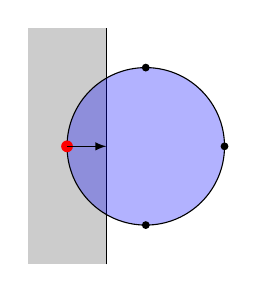
\begin{tikzpicture}[x=10mm,y=10mm]

    % Wall
    \fill[black!20!white] (-1.5, -1.5) rectangle (-0.5, 1.5);
    \draw (-0.5, -1.5) -- (-0.5, 1.5);

    % Ball
    \draw[fill=blue, fill opacity=0.3] (0, 0) circle (1);
    \node[fill, circle, inner sep=1pt] at ( 1, 0) {};
    \node[fill=red, circle, inner sep=1.5pt] at (-1, 0) {};
    \node[fill, circle, inner sep=1pt] at (0,  1) {};
    \node[fill, circle, inner sep=1pt] at (0, -1) {};

    % Arrow
    \draw[->,>=latex] (-1, 0) -- +(0.5, 0);
    \end{tikzpicture}
    \hspace{3em}
}
\hspace{1em}
\subfloat[Second collision check with the ball colliding with a wall corner]{
    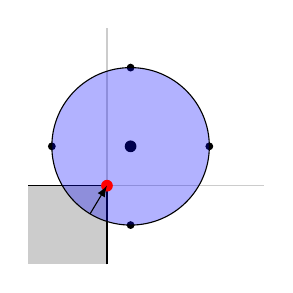
\begin{tikzpicture}[x=10mm,y=10mm]

    % Wall
    \fill[opacity=0.2] (-1.5, -1.5) rectangle (-0.5, -0.5);
    \draw[opacity=0.2] (-0.5, -1.5) -- (-0.5, 1.5);
    \draw[opacity=0.2] (-1.5, -0.5) -- (1.5, -0.5);
    \draw (-0.5, -1.5) -- (-0.5, -0.5) -- (-1.5, -0.5);

    % Ball
    \path (-0.2, 0) node[fill, circle, inner sep=1.5pt] (center) {}
        +(1, 0) coordinate (p)
            node[fill, circle, inner sep=1pt] at +( 1, 0) {}
            node[fill, circle, inner sep=1pt] at +(-1, 0) {}
            node[fill, circle, inner sep=1pt] at +(0,  1) {}
            node[fill, circle, inner sep=1pt] at +(0, -1) {};
    \node(ball) at (center)[draw, fill=blue, fill opacity=0.3, circle through=(p)] {};
    \node[fill=red, circle, inner sep=1.5pt] (corner) at (-0.5, -0.5) {};
    %\node[fill=red, circle, inner sep=1.5pt] (inwall) at (-1, -1) {};
    %\draw[opacity=0.1] (center) -- (inwall);


    % Arrow
    \draw[->,>=latex] (intersection of center--corner and ball) -- (-0.5, -0.5);
    \end{tikzpicture}
    \hspace{3em}
}
\subfloat{
    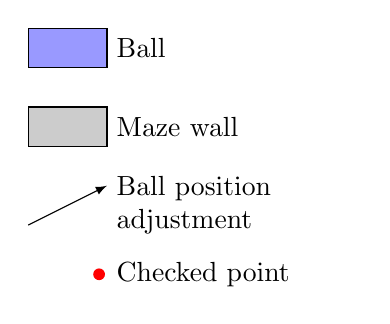
\begin{tikzpicture}[x=10mm,y=-5mm]

    \draw[fill=blue, fill opacity=0.4] (0, 0) rectangle +(-1, 1) +(0, .5)
        node[right, fill opacity=1] {Ball};
    \draw[fill, fill opacity=0.2] (0, 2) rectangle +(-1, 1) +(0, .5)
        node[right, fill opacity=1] {Maze wall};
    \draw[<-,>=latex] (0, 4) -- +(-1, 1); \draw (0, 4.5)
        node[right,text width=3cm, text badly ragged] {Ball position adjustment};
    \path(-0.1, 6.25) node[fill=red, circle, inner sep=1.5pt] {} +(0.1, 0)
        node[right] {Checked point};

    \end{tikzpicture}
}
\caption{Ball collision detection}
\label{fig:collision-detection}
\end{figure}

\subsubsection{Logging and Replaying}

Game logging works by recording which game is played, the state of the random
number generator (RNG), all touch events, and clock ticks.

The logger utilizes Python's \texttt{pickle} module, which allows serializing
arbitrary objects.
“Pickled” messages are compressed and written to a log file, each prefixed by
a short string that names the type of the message.

The first message written is the initial state of the RNG.
Python uses the Mersenne Twister, a pseudo-random number generator whose state
can be stored and later restored to provide an identical sequence of
pseudo-random numbers.

The second message written to the log file is the class of the main game
widget.
This allows the replay script to play either a Maze or a Towers game,
as well as any game written in the future that uses the logging system.
The only requirement is that the game may not use any input or sources of
non-determinism other than what is logged.

After the two initial messages, clock ticks and touch events are recorded as
they happen.

Kivy provides a Clock utility that allows scheduling events and animations.
These events, as well as all graphics, are handled at discrete points in time
called \emph{frames}.
Usually the games run roughly at a fixed frame rate.
In the default Kivy configuration, this is 30 frames per second (FPS).
If processing of a frame takes too much time, the frame rate may drop.
Since some of the game logic depends in subtle ways on the exact points in time
when frames are handled, every frame causes a message containing the time from
the previous frame to be logged.

Finally, whenever an input event occurs, its parameters recorded as well.
Kivy provides three types of touch events: \emph{touch down}, which occurs
whenever a finger touches the surface, \emph{touch move}, which is fired when
a finger already touching the surface is moved, and \emph{touch up}, which
occurs when a finger is lifted.
Each touch has properties such as current position, previous position, and a
unique ID.
All of these properties are recorded when an input event occurs.

When a game is replayed from a log file, the events are read back from the
file, “unpickled”, and processed according to their type.
Meanwhile, all normal touch input (i.e. actual touches, not events from the
log), is redirected to speed up or slow down the replay,
instead of controlling the game.
Because Kivy's Clock utility only uses the real system time, the clock module
is modified while the replay runs to use a customized function of Python's
\texttt{time.time}.
This function synchronizes the clock tick messages and the real clock time.

\section{Hardware}
\label{hw}

As part of the IT project, a prototype touchscreen was built.
This section describes the design, operation, and flaws of the touchscreen.

Figure~\ref{fig:hw-schem} shows a diagram of the touchscreen, and
figure~\ref{fig:hw-photos} shows photos of the finished table.

\begin{figure}[p]
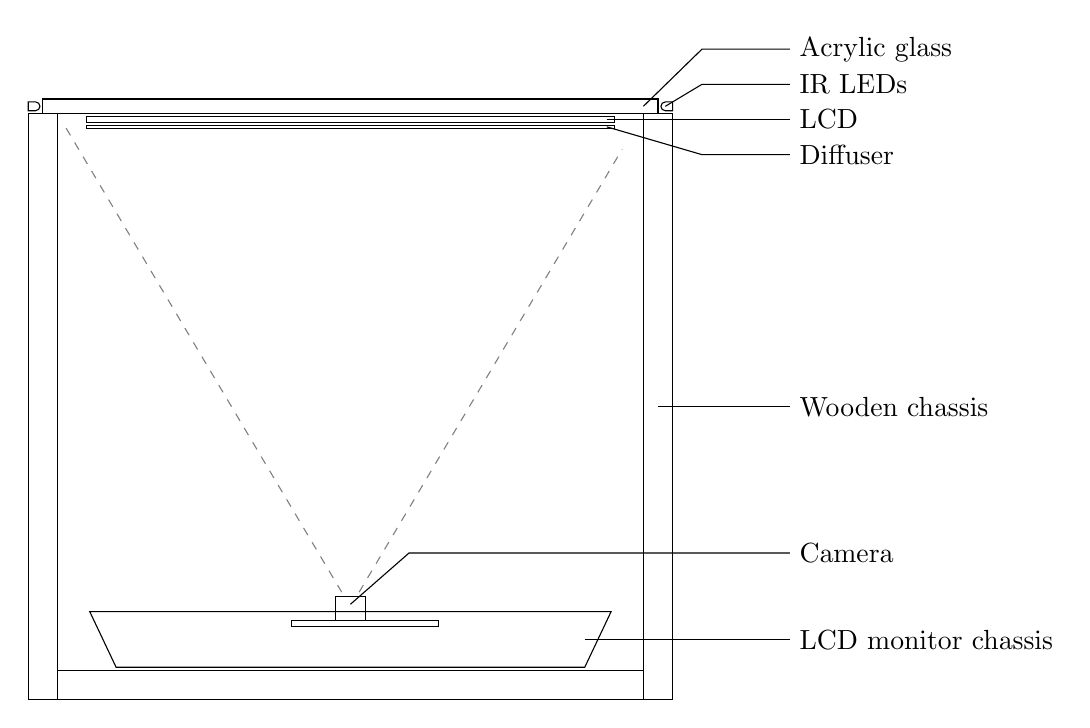
\begin{tikzpicture}[x=4mm,y=4mm,scale=0.93]
\draw (-.5,0) rectangle (20.5,.5); % acrylic
\draw (-1,0) rectangle (0,-20); % front wood
\draw (20,0) rectangle (21,-20); % back wood
\draw (0,-19) rectangle (20,-20); % bottom wood
\draw (1,-.1) rectangle (19,-.3); % LCD
\draw (1,-.4) rectangle (19,-.5); % diffuser
\draw (1.1,-17) -- (18.9,-17) -- (18,-18.9) -- (2,-18.9) -- cycle; % backlight
\draw (9.5,-16.5) rectangle (10.5,-17.3); % camera lens
\draw (8,-17.3) rectangle (13,-17.5); % camera body

\draw (-1,.1) -- (-.75,.1) arc (-90:90:.15) -- (-1,.4) -- cycle; % LED 1
\begin{scope}[xscale=-1,xshift=-80mm]
\draw (-1,.1) -- (-.75,.1) arc (-90:90:.15) -- (-1,.4) -- cycle; % LED 2
\end{scope}

\draw (20,.25) -- (22,2.2) -- (25,2.2) node[right] {Acrylic glass};
\draw (20.75,.25) -- (22,1) -- (25,1) node[right] {IR LEDs};
\draw (18.75,-.2) -- (22,-.2) -- (25,-.2) node[right] {LCD};
\draw (18.75,-.45) -- (22,-1.4) -- (25,-1.4) node[right] {Diffuser};
\draw (20.5,-10) -- (25,-10) node[right] {Wooden chassis};
\draw (10,-16.75) -- (12,-15) -- (25,-15) node[right] {Camera};
\draw (18,-17.95) -- (25,-17.95) node[right] {LCD monitor chassis};

% camera view lines?
\draw[gray,dashed,shorten >=5pt,shorten <=2pt] (9.8,-16.5) -- (0, 0);
\draw[gray,dashed,shorten >=15pt,shorten <=2pt] (10.2,-16.5) -- (20, 0);

\end{tikzpicture}
\caption{Schematic diagram of the touchscreen}
\label{fig:hw-schem}
\end{figure}

\begin{figure}[p]
\subfloat[Front view of the inside]{
    \label{fig:box-front}\includegraphics[width=6.5cm]{box-open-front}}
\hspace{1em}
\subfloat[Touchscreen in action]{
    \label{fig:box-top}\includegraphics[width=6.5cm]{IMG_0950}}
\caption{Photographs of the touchscreen}
\label{fig:hw-photos}
\end{figure}

\subsection{Operation and Construction}

The touchscreen takes advantage of an optical phenomenon called
\emph{frustrated total internal reflection} (FTIR).
Light from infrared light-emitting diodes (LEDs) shines into a sheet of acrylic
glass.
Normally, this light is reflected repeatedly at the acrylic-air boundaries, so
that it effectively stays inside the acrylic.
When a finger is brought within a few wavelengths from the acrylic, it causes
the light to scatter away from the finger.

A camera placed behind the sheet of acrylic records the scattered light, and
the resulting image is processed to obtain \emph{blobs}, or areas corresponding
to the individual fingers touching the acrylic.
The particular camera used is a PlayStation Eye, favored by hobbyist
touchscreen builders for its low cost and high frame rate. % XXX: http://wiki.nuigroup.com/Cameras
The camera's infrared-blocking filter was replaced with a filter from an old
remote control.
The original lens was swapped for a wide-angle lens to reduce the needed depth
of the table.

To provide the infrared light, LEDs are soldered to form two strips.
Each strip is wrapped with clear adhesive tape for insulation, then aluminum
tape to reflect as much light as possible into the piece of acrylic.
The side facing the acrylic is kept clear of any tape.

A LCD (liquid crystal display) layer, obtained from a disassembled computer
monitor, is mounted behind the acrylic sheet.
As LCDs are transparent for infrared light, this does not affect the
touch-sensing capabilities of the screen.
However, the screen's backlight is not transparent and needed to be moved
behind the camera.
This results in decreased brightness when compared to a normal LCD.
Due to the construction of the LCD panel used, the camera could be inserted
into the original monitor chassis containing the backlight, with the lens
protruding through a hole in the backlight's diffuser.
The LED strips are wired to the LCD circuit board, sharing power from the
monitor's supply.

A sheet of tracing paper is installed % XXX: ?
behind the LCD. This serves both to blur the image or the camera so that it is
virtually invisible to the user, and in the reverse direction, to blur the
outside environment so that only blobs corresponding to touching fingers
are discernible by the camera.

The device is enclosed in a wooden box that blocks unwanted light from outside
and prevents movement of the camera relative to the display.
A hinged door in the back of the device allows inspection of the internals.
The power adaptor from the LCD monitor is secured inside the enclosure, away
from the backlight, so that the socket for a power cable is accessible.
In addition to the power cable, an USB cable for the camera and a VGA cable
for the monitor extend from the device and need to be connected to the computer
running the games.

\subsection{Problems}

Due to the decreased brightness of the LCD backlight, the touchscreen functions
best in rooms that are not fully lit.
Also, it reacts differently to fingers of different people, or even different
fingers on the same hand, which means that some people may need to press harder
on the screen than others.
An effective way to get fingers registered more reliably is to wet them
slightly before touching the surface.
This limitation might be overcome by using a compliant surface layer, such as
a thin film of transparent silicone, atop the acrylic.
However, such a solution would be fairly expensive and risky, as the layer
needs to be even so as to not distort the LCD image.

The firmware and drivers for the PS3 Eye camera are designed to adapt to
lighting conditions.
Whenever such an adaptation occurs, “fake” tou\-ches may start being registered
or legitimate touches may be missed.
Keeping the table and room lit by a stable overhead light source helps prevent
this problem.

Despite these shortcomings, the table is usable and according to user testing,
the games played on it are quite engaging.

\end{document}

\section{Future Work}

The games and the touch table will be used in an study exploring
the usability of multi-touch input in games.
The touchscreen will be also used, preferably in addition to a larger table
that is currently being built in the department.

% XXX: Refer to all figures

